% !TEX root = ../thesis.tex

\chapter{Two-Qubit Gates for the Soft \zps Qubit}\label{apx:chp_zero_pi}

\section{Single-Qubit Simulation Details}\label{zp:app:1Qgate_simulation}
The software used to generate the figures in this chapter is available in our open-source GitHub repository \cite{zp2q_repo}.
Note that we use the ``scQubits'' Python package to construct the single- and two-qubit Hamiltonians \cite{groszkowskiScqubitsPythonPackage2021a,chittaComputeraidedQuantizationNumerical2022a}.
This section outlines the numerical techniques used in the single-qubit simulations.
For more details, please refer to the source code.

\subsection{Noiseless simulation of single-qubit gates}
To simulate the \zps qubit, we numerically diagonalize the Hamiltonian in \cref{zp:eq:zp Hamiltonian} and keep the lowest $N_{\rm max} +1$ energy levels.
Before diagonalization, we construct operators for the $\theta$ mode in the charge basis and for the $\phi$ mode in the phase basis with $\phi \in \left[-6\pi, 6\pi \right]$.
We set the dimensions of these bases to 181 and 300, respectively.
Numerical simulations with larger truncations show that the qubit frequency (the eigenvalue of $\ket{2}$) converges to within $\sim 10^{-8}$ GHz when either basis is reduced by 5.
For the highest retained state ($N_{\rm max}=299$), the corresponding maximum change is $\sim 10^{-5}$ GHz.
In the diagonal basis, the \zps Hamiltonian is
\begin{equation}
H_{0\text{-}\pi} = \sum_{p=0}^{N_{\rm max}} \omega_{0 \text{-} p} \ket{p} \bra{p},
\end{equation}
where $\ket{p}$ is an eigenvector with eigenvalue $\hbar \omega_{0 \text{-} p}$ (with $\hbar=1$).
To add the drive, we express the operator $n_{\rm op}$ with ${\rm op} \in \{\theta, \phi\}$ in the diagonal basis of the \zps Hamiltonian as $n_{\rm op} = \sum_{i,j=0}^{N_{\rm max}} n^{i \text{-} j}_{\rm op} \ket{i} \bra{j}$, where $n^{i \text{-} j}_{\rm op} = \bra{i} n_{\rm op} \ket{j}$ and $\ket{i}, \ket{j} \in \{\ket{p}\}$.

Leakage from the computational subspace into higher excited states is a known issue for the \zps qubit~\cite{PremkumarAPS2023,premkumar2023hamiltonian}.
We therefore verify that our finite-level truncation faithfully approximates the dynamics of a converged larger model.
We first increase the truncation size $n$ in increments of 100 and calculate the corresponding gate fidelity $F_n$.
We assess convergence from the change in infidelity between successive truncations by requiring
$|(1-F_n)-(1-F_{n-100})|\leq (1-F_n)/10,$
such that the truncation-induced change is at least one order of magnitude smaller than the infidelity itself.
For example, if $1-F_n=10^{-3}$, we require the change relative to the calculation with $n-100$ states to be no greater than $10^{-4}$.
The largest model, with $N_{\rm max}=1000$ states, satisfies this convergence criterion and serves as the reference.
We then compare calculations with smaller truncations against the $N_{\rm max}=1000$ result to identify the smallest model that reproduces the reference infidelity to the same level of accuracy.
Using this procedure, we find that $N_{\rm max}=300$ states is sufficient for the single-qubit gate simulations.

We also control integration error using QuTiP’s propagator routine.
The time-step convergence criterion is similar to that for truncation.
We chose the maximum time step so that increasing it by approximately a factor of three changed the infidelity by less than one tenth of the infidelity itself.
Thus we used a maximum step size of $\Delta t_{\rm max}=3\times10^{-4}$ ns for $n_\theta$ drives and $1\times10^{-3}$ ns for $n_\phi$ drives in our simulations.

\subsection{Model reduction for noiseless pulse optimization}
\label{zp:app:sec:model_reduce_1q}
Modeling the \zps requires a large Hilbert space, making simulations slow.
Optimizing pulse parameters requires solving the dynamics many times.
To balance speed and accuracy, we construct a reduced model for pulse optimization in the \zps qubit.
The reduced model includes only states accessible from the logical subspace under the chosen drive.

We build the reduced model by first including the logical states $\ket{0}$ and $\ket{2}$, and the intended intermediate state ($\ket{7}$ for $n_\theta$, $\ket{9}$ for $n_\phi$).
The drive operator $n_{\rm op}$ with ${\rm op} \in \{\theta, \phi\}$ couples the states in the current reduced model to other states in the Hilbert space.
Next we compute matrix elements $n_{\rm op}^{i\text{-}j}=\bra{i}n_{\rm op}\ket{j}$ for all $\ket{i}$ in the reduced model and $\ket{j}$ outside it.
Any state $\ket{j}$ with $|n_{\rm op}^{i\text{-}j}|\geq n_{\rm thresh}$ is absorbed into the model.
Repeating this procedure over the lowest 300 states yields a stable reduced model once no further states are added.
We call the resulting set the selected states.
For thresholds $n_{\rm thresh}\in[10^{-8},0.2]$, the same reduced models emerge, containing 157 states for $n_\theta$ and 160 for $n_\phi$.

Even with a reduced Hilbert space, simulations remain costly.
We gain further efficiency by evolving only the logical states instead of the full propagator.
By default, QuTiP v4.7 evolves all basis states, which is unnecessary for gate fidelity optimization.
Restricting to logical states greatly speeds up simulations, allowing a 100-ns $X$ gate in a $\sim$200-state space to be optimized in about 1 hour using 30 AMD EPYC 7713 cores.

\subsection{Single-qubit pulse optimization}\label{zp:app:sub_sec_pluse_opt}
\begin{figure}[htbp]
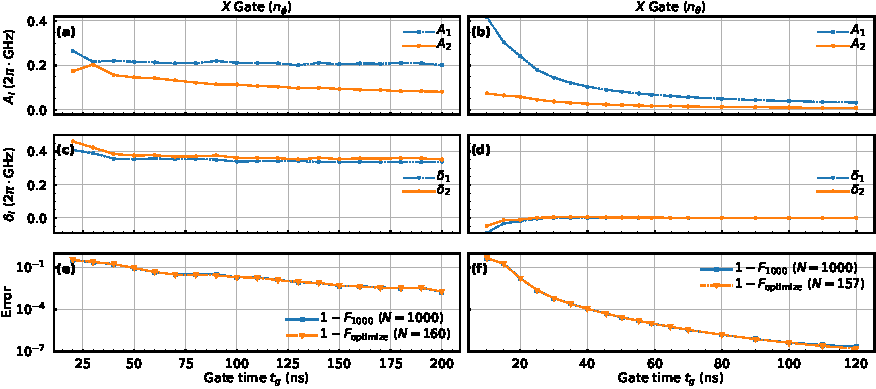
\includegraphics[width=\textwidth]{chapter-4-zero-pi/figs/params_1q.pdf}
\centering
\caption[Optimized single-qubit pulse parameters.]{
Optimized pulse parameters and gate infidelities for an $X$ gate driven through $n_{\rm op}$, with ${\rm op}\in\{\phi,\theta\}$.
For each gate time $t_g$, panels (a,b) show the optimized amplitudes $(A_1,A_2)$, panels (c,d) show the optimized detunings $(\delta_1,\delta_2)$, and panels (e,f) show the corresponding infidelities.
The pulses are optimized in a closed-system truncated model with $N_{\rm optimize}=160$ levels for the $n_\phi$ drive and $N_{\rm optimize}=157$ levels for the $n_\theta$ drive.
The resulting fidelity is $F_{\rm optimize}$.
The same pulses are then tested in a closed-system 1000-level model, giving $F_{1000}$.
}
\label{zp:fig:params_1q}
\end{figure}
To construct an $X$ gate, we use an effective $\Lambda$ system driven on both legs, which unavoidably introduces some leakage.
The drive Hamiltonian in \cref{zp:eq:zp_H_drive}, with Gaussian envelopes defined in \cref{zp:eq:gauss_envelope}, is specified by five parameters: gate time $t_g$, amplitudes $A_{1,2}$, and detunings $\delta_{1,2}$.
With $t_g$ fixed (tolerance $\pm0.1$ ns), only four parameters are optimized.

Given the pulse parameters, we numerically solve the Schr\"odinger equation,
\begin{equation}
i \frac{\partial V(t)}{\partial t} = \left(H_{0\text{-}\pi} + H_{\rm drive}\right) V(t),
\end{equation}
with $V(0)=I$, to obtain the evolution operator $V(t)$.
Gate quality is measured by the average fidelity between the target unitary $U_{\rm targ}$ ($=X$) and the simulated propagator $V$ in the logical subspace $\{\ket{0},\ket{2}\}$:
\begin{equation}
F(U_{\rm targ},V)=
\frac{
\operatorname{Tr}(V^\dagger V) +
\big| \operatorname{Tr}(U_{\rm targ}^\dagger V) \big|^2
}
{d(d+1)}\,,
\label{zp:eq:gate_fidelity}
\end{equation}
with $d = 2$.
For improved numerical behavior, we optimize over the quantity $\log_{10}(1 - F)$.
Due to leakage, $V$ is generally not unitary, although it is close to unitary for high-fidelity operations.

The optimization is constrained by $A_i/2\pi \in (0,\ 500)\ \text{MHz}$ and $\delta_i/2\pi \in (-500,\ 500)\ \text{MHz}$.
We first optimize in the reduced model from \cref{zp:app:sec:model_reduce_1q}, then re-run the search using the result as an initial guess to avoid local minima.
The optimization uses ``differential evolution'', a gradient-free stochastic method~\cite{storn1997differential} that efficiently explores large parameter spaces in parallel.
Finally, we validate the optimized pulse by simulating the system in a larger Hilbert space spanned by the lowest 1000 eigenstates.

After each optimization, we record the infidelity and use the result as the initial guess for the next iteration to improve convergence.
This process is repeated for all gate times.
The optimized pulse parameters obtained for the previous gate time are used as the initial guess for the optimization at the next gate time.
This warm-start strategy significantly accelerates the optimization.

In \cref{zp:fig:params_1q}, we show the optimized pulse parameters and gate infidelity for the $X$ gate with $n_\theta$ and $n_\phi$ drives.
Panels (a)–(b) display the drive amplitudes.
The amplitude ratio $A_1/A_2$ is largely set by the ratio of charge matrix elements $n_{\rm op}^{2\text{-}i}/n_{\rm op}^{0\text{-}i}$.
In an ideal three-level $\Lambda$ system these ratios coincide, giving the fastest transfer.
Due to transitions nearby in a large Hilbert space, we need to optimize $A_1$ and $A_2$ independently.
For the optimized pulse parameters shown in \cref{zp:fig:params_1q}, the amplitude ratio  $A_1/A_2$ agrees well with the matrix element ratio, $n_{\rm op}^{2\text{-}i} / n_{\rm op}^{0\text{-}i}$ for $n_\theta$ driving.
This agreement does not hold for $n_\phi$ driving.
However, the ratio of the drive amplitudes converges closely to the ratio of the charge matrix elements as the gate time increases beyond 200 ns for $n_\phi$ driving.
This is also the case for the $\sim$800 ns $X$ gate, achieved via driving $n_\phi$, presented in \cref{zp:sec:x_gate_reproduce}.
Also visible in (b) is the decrease in amplitudes with gate time, which correlates with reduced gate error in (f).
Panels (c)–(d) show the detunings, indicating off-resonant vs. resonant driving for $n_\phi$ and $n_\theta$.
Panels (e)–(f) show gate infidelities for the full model with 1000 states ($1-F_{n_{\rm op}}$) and two reduced models.

To get an idea of the order of magnitude of the error incurred by truncation,  we also compute the relative gate-error difference $|F_{1000}-F_{\rm optimize}|/(1-F_{1000})$ in \cref{zp:fig:params_1q}(e)–(f).
For $n_\theta$ driving, the average and maximum differences are $1.16\times10^{-2}$ and $5.56\times10^{-2}$, respectively.
For $n_\phi$ driving, they are $4.59\times10^{-2}$ and $1.47\times10^{-1}$.

\subsection{Noisy simulation of single-qubit gates}\label{zp:app:sub_sec_noisy_1Q}
We simulate noise using the master equation $\dot\rho=\mathcal{L}[\rho]$, whose solution is $\rho(t)=e^{\mathcal{L}t}[\rho(0)]$, with $e^{\mathcal{L}t}$ the propagator from $\rho(0)$ to $\rho(t)$.
The noise model includes energy relaxation ($T_1$) and pure dephasing ($T_\phi$), with equal characteristic times $T_1=T_\phi=T$.
We consider $T\in\{3,30,170\}\,\mu\mathrm{s}$.
These values are chosen to represent noise regimes corresponding approximately to gate fidelities of $\sim99\%$, $\sim99.9\%$, and above $99.9\%$, respectively.

To compute gate fidelities, we fix a target gate time and use the noiselessly optimized pulse parameters (drive frequencies and amplitudes).
We then integrate the master equation to obtain the superoperator propagator $\tilde{\mathcal{X}}=e^{\mathcal{L}t}$, with Liouvillian $\mathcal{L}$.
At the final time, $\tilde{\mathcal{X}}$ is converted into Kraus operators $V_k$, defining the noisy channel $V(\rho)=\sum_k V_k \rho V_k^\dagger$.
The average channel fidelity relative to the target $X$ gate is then
\begin{equation}
F(U_{\rm targ},V)
\!=\!
\frac{1}{d(d+1)}
\displaystyle
\sum_k \left[
\operatorname{Tr}(V_k^\dagger V_k) +
\big| \operatorname{Tr}(U_{\rm targ}^\dagger V_k)
\big|^2 \right],
\label{zp:eq:channel_fidelity}
\end{equation}
with $U_{\rm targ}=X$ and $d=2$.
Because energy-relaxation rates scale with charge matrix elements, they vanish when the matrix element is negligible.
Because open-system simulations are computationally more demanding, we employ a smaller Hilbert-space truncation than in the corresponding closed-system simulations.
For noisy single-qubit simulations, we evolve the optimized pulse in a reduced subspace of $N$ selected states, with $N=160$ for the $n_\phi$ drive and $N=157$ for the $n_\theta$ drive.
The resulting superoperator is then used to compute the noisy channel fidelity relative to the ideal $X$ gate.

\section{Comparison to Experimental Single-Qubit Gate Performance}
\label{zp:sec:x_gate_reproduce}

To validate our methods, we simulate a gate similar to the $X$ gate demonstrated in Ref.~\cite{Gyenis_zero_pi_2021a}.
It used a Gaussian pulse with detuning $\delta\approx-4$ MHz and $\sigma=200$ ns, so $t_g\approx800$ ns.
That gate achieved a fidelity $\leq90\%$ \cite{andras_xgate}.

We already use the same device parameters (such as $E_J$, $E_C$, etc.) as in the experiment.
To replicate their resonator-pin drive, we model the drive operator as $n_{\rm op} \propto b_\phi n_\phi + b_\theta n_\theta$, where the coupling rates are $b_\phi = 0.27$ and $b_\theta = 6.6 \times 10^{-3}$~\cite{Gyenis_zero_pi_2021a}.
With this model, we numerically optimize a pulse and find a gate with $t_{\rm g} \approx 830$ ns, which is of the same order of magnitude as the gate duration in Ref.~\cite{Gyenis_zero_pi_2021a}.
This pulse was optimized on the closed system model, not the open system model.
It would likely be improved by directly optimizing the open system model.

\Cref{zp:fig:exp_gate_population} shows the noiseless population transfer for this gate.
With parameters $A_1=13.56$ MHz, $A_2=34.96$ MHz, $\delta_1=-3.03$ MHz, $\delta_2=-3.18$ MHz, and $t_g=828.76$ ns, we obtain a noiseless fidelity of $F=99.85\%$.
Including noise with $T_1=T_\phi=3\ \mu$s reduces the fidelity to $F=85.72\%$, which is comparable to the experimental value.
This demonstrates that our model captures key features of the experimental gate.

\begin{figure}[htbp]
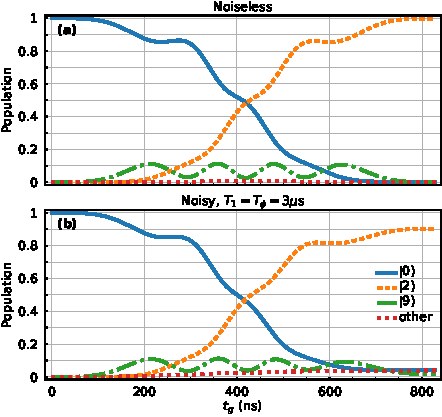
\includegraphics[width=\colfigwidth]{chapter-4-zero-pi/figs/xgate_population_phi+theta_2panels.pdf}
\centering
\caption[Population transfer in a simulated gate comparable to experiment.]{
Population transfer during an $X$ gate with $t_{\rm g}=828.76$ ns, driven by $n_{\rm op} \propto b_\theta n_\theta + b_\phi n_\phi$.
(a) Noiseless simulation with fidelity $F=99.85\%$.
(b) Noisy simulation with $T_1=T_\phi=3~\mu$s, reducing fidelity to $F=85.72\%$.
The experimental drive coefficients were $b_\theta=6.6\times10^{-3}$ and $b_\phi=0.27$.
For consistency with the $n_\phi$ and $n_\theta$ driving in the main text, we normalize these coefficients while preserving their ratio, giving $n_{\rm op}=0.976\, n_\phi+0.024\,n_\theta$ in the simulations.
}\label{zp:fig:exp_gate_population}
\end{figure}

There is an apparent discrepancy between the gate times studied here and those in the main text.
The gate in this section is significantly slower, and its closest counterpart in the main text is the $n_\phi$-driven gate.

The main reason is the much larger effective Rabi rates achievable in our protocol.
Ref.~\cite{Gyenis_zero_pi_2021a} demonstrated Raman control with effective Rabi frequencies of only a few MHz.
However, this limitation was not intrinsic to the soft 0-$\pi$ qubit itself.
Rather, as noted in Ref.~\cite{Gyenis_zero_pi_2021a}, the control tones were applied through the readout cavity, whose strong filtering substantially reduced the drive power reaching the qubit.
In contrast, our simulations assume direct microwave control and exploit intermediate states with relatively large transition matrix elements.
The optimized parameters in \cref{zp:tab:xgate_parameters} yield effective single-photon Rabi rates up to $\Omega/2\pi \approx 60~\mathrm{MHz}$, approximately an order of magnitude larger than those reported experimentally.
These larger effective Rabi rates are a major factor behind the significantly shorter gate times found in the main text.

A second difference is the drive operator.
In this section, the drive has the form $b_\phi n_\phi + b_\theta n_\theta$, whereas the main text studies gates driven by $n_\phi$ or $n_\theta$ alone.
Simulations not shown here indicate that driving the combined operator $b_\phi n_\phi + b_\theta n_\theta$ produces more leakage than driving either operator
alone.
These additional leakage pathways reduce the gate fidelity and likely contribute to the slower gate in Ref.~\cite{Gyenis_zero_pi_2021a}.

Finally, there are likely differences associated with noise and leakage modeling.
Our model captures key experimental features, but it is not a complete device-level model.
In particular, our model does not include a $\zeta$ mode, and higher excited states may decohere more strongly in the experiment than assumed in our simulations.
The main-text $n_\phi$ gate also reaches a larger intermediate-state population than the gate in this appendix, with $P_9\sim 0.22$ compared with $P_9\sim 0.12$.
Reducing this population is possible, but generally requires longer gate times.
For comparison, the simulation in Appendix G of Ref.~\cite{Gyenis_zero_pi_2021a} shows an intermediate-state population of approximately $5.5\%$ in Fig.~16(e), likely due to the use of an effective three-level Hilbert space in that calculation.

After submission, we became aware of the thesis by \citet{premkumar2023hamiltonian}.
We do not directly compare our model with the results in Fig.~4.9 of the thesis because the simulations differ in several important respects.
In particular, the simulated device uses parameters that differ substantially from those of Ref.~\cite{Gyenis_zero_pi_2021a}, the gate employs a flat-top Gaussian pulse rather than the pulse considered here, and the two Raman tones are constrained to have a common detuning from their respective transitions.
By contrast, we optimize the two drive detunings independently.

\section{Quantization of two coupled \texorpdfstring{\zp}{zero-pi} qubits }\label{zp:app:quantize}

In \cref{zp:app:coupling_scheme_theta} we first quantize the circuit in \cref{zp:fig:circuit_2qubits}(a), which produces an  $ n_{\theta1} n_{\theta 2} $ coupling.
We then quantize the circuit in \cref{zp:fig:circuit_2qubits}(b), which produces an  $ n_{\theta1}n_{\theta2} - n_{\phi1}n_{\phi2} $  coupling.

\subsection{Pure coupling scheme: \texorpdfstring{$ n_{\theta1} n_{\theta 2} $} {theta} }\label{zp:app:coupling_scheme_theta}

Our goal is to quantize the 10-node circuit in \cref{zp:fig:circuit_2qubits} (a).
The derivation below assumes equal capacitances for both \zps circuits.
If we instead allowed different capacitances for the two qubits, the coupling strength and $\theta$ mode capacitance would be slightly modified.
Crucially, this does not change the circuit quantization procedure, variable transformation, or the form of the effective Hamiltonian.

Let $T_{0\text{-}\pi}^{(i)}$ and $U_{0\text{-}\pi}^{(i)}$ denote the kinetic (capacitive) and potential terms of the Lagrangian for the $i^\text{th}$ \zps qubit, respectively, where $i \in \{1, 2\}$.
Let $T_{\rm int}$ represent the interaction between the two qubits.
Then, the full system Lagrangian is
\begin{align}\label{zp:eq:full_sys_lagrangian}
\mathcal{L}
=& \sum_{i=1,2}{(T_{0\text{-}\pi}^{(i)} - U_{0\text{-}\pi}^{(i)} )} + T_{\rm int} \, .
\end{align}
Here, the superscript $i\in\{1,2\}$ labels the qubit, and $T_{\rm int}$ represents the interaction between the two \zps qubits.
$T_{0\text{-}\pi}^{(i)}$ and $U_{0\text{-}\pi}^{(i)} $ are the kinetic and potential parts of the single-qubit Lagrangian, respectively.
The kinetic terms for the two \zps qubits are
\begin{widetext}
\begin{align}
T_{0\text{-}\pi}^{(1)}
&= (C+C_{J})\dot{\theta}_1^2 +  C_J\dot{\phi}_1^2 + C\dot{\zeta}_1^2 + \half C_0 \sum_{i=1}^{4}{\dot{\varphi}_i^2} \nonumber\\
& =  ( C+C_J+\half C_0  ) \dot{\theta}_1^2 +  (C_J+\half C_0) \dot{\phi}_1^2 + ( C+\half C_0 ) \dot{\zeta}_1^2 +\half C_0  \dot{\Sigma}_1^2,  \\
T_{0\text{-}\pi}^{(2)}
&= (C+C_{J})\dot{\theta}_2^2 +  C_J\dot{\phi}_2^2 + C\dot{\zeta}_2^2 + \half C_0  \sum_{i=5}^{8}{\dot{\varphi}_i^2} \nonumber \\
&= ( C+C_J+\half C_0 ) \dot{\theta}_2^2 +  (C_J+\half C_0) \dot{\phi}_2^2 + ( C+\half  C_0 ) \dot{\zeta}_2^2 +\half C_0 \dot{\Sigma}_2^2 \, .
\end{align}
In these expressions, the top line has the node variables and the bottom line is re-expressed with respect to our variable transformation in \cref{zp:eq:zp_transform}.
The additional terms relative to the single \zps circuit, proportional to $C_0$, arise from the ground capacitors.
The coupling term is more complicated and can be written as
\begin{align}
T_{\rm int}
&=\frac{C_{c}}{2}
[(\dot{\varphi }_1-\dot{\varphi }_{10}){}^2 +
(\dot{\varphi }_4-\dot{\varphi }_{10}){}^2 +
(\dot{\varphi }_5-\dot{\varphi }_{10}){}^2 +
(\dot{\varphi }_8-\dot{\varphi }_{10}){}^2 \nonumber
\\
&\quad +(\dot{\varphi }_2-\dot{\varphi }_9){}^2 +
(\dot{\varphi }_3-\dot{\varphi }_9){}^2 +
(\dot{\varphi }_6-\dot{\varphi }_9){}^2 +
(\dot{\varphi }_7-\dot{\varphi }_9){}^2]  \nonumber
\\
&= \frac{C_{c}}{2} \Big [ \sum_{i=1}^{8}{\dot{\varphi}_i^2}
+ 4(\dot{\varphi}_9^2 + \dot{\varphi}_{10}^2)
-2\dot{\varphi}_9 (\dot{\varphi}_2 + \dot{\varphi}_3 + \dot{\varphi}_6 + \dot{\varphi}_7)
-2\dot{\varphi}_{10} (\dot{\varphi}_1 + \dot{\varphi}_4 + \dot{\varphi}_5 + \dot{\varphi}_8) \Big ]   \nonumber
 \\
&=\frac{C_c}{2}\sum_{i=1}^{2} [\dot{\phi}_i^2 + \dot{\zeta}_i^2
+(\dot{\varphi }_+ - \dot{\Sigma }_i)^2
+(\dot{\varphi }_- - \dot{\theta }_i)^2 ] \, .
\end{align}
The final line is written using the variable transformation in \cref{zp:eq:zp_transform} and the sum and difference variables
$\varphi_{\pm}=\varphi_9\pm\varphi_{10}$.
Finally, the potential term is
\begin{equation}
U_{0\text{-}\pi}^{(i)}
=-2E_{Ji} \cos{\theta_i} \cos{(\phi_i-\phiext{}_{,i}/2)} + E_{Li}\phi_i^2 + E_{Li} \zeta_i^2 .
\end{equation}
After doing the Legendre transform, the vector of conjugate momenta $Q_\mu=\partial\mathcal{L}/\partial\dot{\mu}\ (\mu=\theta_j,\phi_j,\zeta_j,\Sigma_j,+,-;\ j=1,2)$ is
\begin{align} \label{zp:eq:capacitance_mat1}
\left(\begin{array}{c}
Q_{\theta 1} \\
Q_{\Sigma 1} \\
Q_{\phi 1} \\
Q_{\zeta 1} \\
Q_{\theta 2} \\
Q_{\Sigma 2} \\
Q_{\phi 2} \\
Q_{\zeta 2} \\
Q_{+}\\
Q_{-}
\end{array}\right)=\left(\begin{array}{cccccccccc}
C_\theta & 0 & 0  & 0 & 0  & 0 & 0  & 0 & 0  & -C_c \\
0 & C_\Sigma & 0  & 0 & 0  & 0 & 0  & 0 & -C_c  & 0 \\
0 & 0 & C_\phi  & 0 & 0  & 0 & 0  & 0 & 0  & 0 \\
0 & 0 & 0  & C_\zeta & 0  & 0 & 0  & 0 & 0  & 0 \\
0 & 0 & 0  & 0 & C_\theta  & 0 & 0  & 0 & 0  & -C_c \\
0 & 0 & 0  & 0 & 0  & C_\Sigma & 0  & 0 & -C_c  & 0 \\
0 & 0 & 0  & 0 & 0  & 0 & C_\phi  & 0 & 0  & 0 \\
0 & 0 & 0  & 0 & 0  & 0 & 0  & C_\zeta & 0  & 0 \\
0 & -C_c & 0  & 0 & 0  & -C_c & 0  & 0 & 2C_c  & 0 \\
-C_c & 0 & 0  & 0 & -C_c  & 0 & 0  & 0 & 0  & 2C_c
\end{array}\right)\left(\begin{array}{c}
\dot{\theta}_1 \\
\dot{\Sigma}_1 \\
\dot{\phi}_1 \\
\dot{\zeta}_1 \\
\dot{\theta}_2 \\
\dot{\Sigma}_2 \\
\dot{\phi}_2 \\
\dot{\zeta}_2 \\
\dot{\varphi}_+\\
\dot{\varphi}_-
\end{array}\right) \, .
\end{align}
In the above equation, the capacitances $C_{\mu}$ of the \zps qubit modes  for $\mu \in \{\theta,\ \phi,\ \zeta,\ \Sigma\}$ are specified by
\begin{align} \label{zp:eq:capacitance_transform}
\left(\begin{array}{c}
C_{\theta} \\
C_{\phi} \\
C_{\zeta} \\
C_{\Sigma} \\
\end{array}\right)=\left(\begin{array}{cccc}
2 & 2 & 1 & 1  \\
0 & 2 & 1 & 1  \\
2 & 0 & 1 & 1  \\
0 & 0 & 1 & 1  \\
\end{array}\right)\left(\begin{array}{c}
C \\
C_J \\
C_c \\
C_0 \\
\end{array}\right) \,
\end{align}
where $C_0$ is the capacitance between the node and ground.
With a less intuitive choice of intermediate variables,
\begin{equation}
    \varphi_+' = \varphi_+-(\Sigma_1+\Sigma_2)/2\quad \text{and}\quad \varphi_-' = \varphi_--(\theta_1+\theta_2)/2,
\end{equation}
the coupling between the $\theta$ and $\Sigma$ modes of the two qubits can be seen directly:
\begin{align} \label{zp:eq:capacitance_mat}
\left(\begin{array}{c}
Q_{\theta 1} \\
Q_{\Sigma 1} \\
Q_{\phi 1} \\
Q_{\zeta 1} \\
Q_{\theta 2} \\
Q_{\Sigma 2} \\
Q_{\phi 2} \\
Q_{\zeta 2} \\
Q_{+'}\\
Q_{-'}
\end{array}\right)=\left(\begin{array}{cccccccccc}
C_\theta-\frac{C_c}{2} & 0 & 0  & 0 & -\frac{C_c}{2}  & 0 & 0  & 0 & 0  & 0 \\
0 & C_\Sigma -\frac{C_c}{2}& 0  & 0 & 0  & -\frac{C_c}{2} & 0  & 0 & 0  & 0 \\
0 & 0 & C_\phi  & 0 & 0  & 0 & 0  & 0 & 0  & 0 \\
0 & 0 & 0  & C_\zeta & 0  & 0 & 0  & 0 & 0  & 0 \\
-\frac{C_c}{2} & 0 & 0  & 0 & C_\theta -\frac{C_c}{2}  & 0 & 0  & 0 & 0  & 0 \\
0 & -\frac{C_c}{2} & 0  & 0 & 0  & C_\Sigma -\frac{C_c}{2}& 0  & 0 & 0  & 0 \\
0 & 0 & 0  & 0 & 0  & 0 & C_\phi  & 0 & 0  & 0 \\
0 & 0 & 0  & 0 & 0  & 0 & 0  & C_\zeta & 0  & 0 \\
0 & 0 & 0  & 0 & 0  & 0 & 0  & 0 & 2C_c  & 0 \\
0 & 0 & 0  & 0 & 0  & 0 & 0  & 0 & 0  & 2C_c
\end{array}\right)\left(\begin{array}{c}
\dot{\theta}_1 \\
\dot{\Sigma}_1 \\
\dot{\phi}_1 \\
\dot{\zeta}_1 \\
\dot{\theta}_2 \\
\dot{\Sigma}_2 \\
\dot{\phi}_2 \\
\dot{\zeta}_2 \\
\dot{\varphi}_+'\\
\dot{\varphi}_-'
\end{array}\right) \, .
\end{align}

Calculating the inverse of the capacitance matrix in \cref{zp:eq:capacitance_mat} gives the total quantized Hamiltonian  $H=\frac{1}{2}Q^TC^{-1}Q + U$, which can be decomposed as
\begin{align}\label{zp:eq:H_tot_apxA1}
    H &= H_{0\text{-}\pi}^{(1)} + H_{0\text{-}\pi}^{(2)} + H_{\rm int} + H_{\rm coupler},
\end{align}
where $H_{\rm int}$ represents the interaction between the two qubit circuits and the coupling circuit, while $H_{\rm coupler}$  is the coupler self-Hamiltonian.
The Hamiltonian of the individual \zps qubits is
\begin{align}\label{zp:eq:zp_h_app_i}
    H_{0\text{-}\pi}^{(i)} &=  4\tilde E_C^{\theta} {n}_{\theta i}^2 + 4\tilde E_C^{\phi} {n}_{\phi i}^2  + 4\tilde E_C^{\zeta} {n}_{\zeta i}^2 + 4\tilde E_C^{\Sigma} {n}_{\Sigma i}^2 +
    E_{Li}{\phi}_i^2 + E_{Li}{\zeta}_i^2 - 2E_{Ji}\cos{{\theta}_i}\cos \Big ({\phi}_i - \frac{\phiext}{2}\Big) ,
\end{align}
where the associated energies are
\begin{subequations}
\begin{align}\label{zp:eq:renormalized_ec}
    \tilde E_{C}^{\theta} &= \frac{e^2(2C_\theta-C_c)}{4C_{\theta}(C_{\theta} - C_c)},
   & \tilde E_{C}^{\phi} &= \frac{e^2}{2C_\phi},
   \\
    \tilde E_{C}^{\Sigma} &= \frac{e^2(2C_\Sigma-C_c)}{4C_{\Sigma}(C_{\Sigma} - C_c)} ,
   & \tilde E_{C}^{\zeta} &= \frac{e^2}{2C_\zeta} \, .
\end{align}
\end{subequations}
The two remaining parts of \cref{zp:eq:H_tot_apxA1} are
\begin{subequations}
\begin{align}
    H_{\rm coupler} = 4E_C^- n_m^2 + 4E_C^+ n_p^2 ,
    \quad {\&}\quad
    H_{\rm int} = g_{\theta} n_{\theta_1}n_{\theta_2} + g_{\Sigma} n_{\Sigma_1}n_{\Sigma_2},
\end{align}
\end{subequations}
with the coefficients
\begin{subequations}\label{zp:eq:coupling_rates_app}
\begin{align}
    g_{\theta} &=\frac{2e^2C_c}{C_{\theta} (C_{\theta} - C_c)} \approx \frac{e^2C_c}{2C^2},
    &E_{C}^{+} &=\frac{e^2}{4C_c},
    \\
    g_{\Sigma} &= \frac{2e^2C_c}{C_{\Sigma}(C_{\Sigma} - C_c)} = \frac{2e^2C_c}{C_0(C_0+C_c)}, &E_{C}^{-} &= \frac{e^2}{4C_c}.
\end{align}
\end{subequations}
The approximate expressions are valid in the limit of $C\gg C_c,C_J,C_0$.
In the above expressions, the modes $\zeta_1$ and $\zeta_2$ are decoupled from the effective modes of the \zps qubit and can thus be considered separately.
The modes $\Sigma_1$, $\Sigma_2$, $\varphi_+$, and $\varphi_-$ do not have corresponding potential energy terms and are considered free modes.
Because they are decoupled from the $\theta, \phi,$ and $\zeta$ degrees of freedom, the free modes may be ignored without affecting the system dynamics.
Thus the final Hamiltonian can be written as
\begin{subequations}
\begin{align}
    H_{\rm tot} &= H_{0\text{-}\pi}^{(1)} + H_{0\text{-}\pi}^{(2)} + H_{\rm int},
    \\
    H_{0\text{-}\pi}^{(i)} &=  4\tilde E_C^{\theta} n_{\theta i}^2 + 4\tilde E_C^{\phi} n_{\phi i}^2   +   E_{Li}\phi_i^2 - 2E_{Ji}\cos{\theta_i}\cos\Big (\phi_i - \frac{\phiext}{2}\Big) ,
    \\
    H_{\rm int} &= g_{\theta} n_{\theta_1}n_{\theta_2}.
\end{align}
\end{subequations}

\subsection{ Mixed coupling scheme: \texorpdfstring{$ n_{\theta1}n_{\theta2} - n_{\phi1}n_{\phi2} $}{theta + phi}}\label{zp:app:coupling_scheme_mix}
Now we quantize the circuit in \cref{zp:fig:circuit_2qubits}(b).
We use the variable transformation in \cref{zp:eq:zp_transform} on both \zps qubits.
The Lagrangian is expressed, as before, in \cref{zp:eq:full_sys_lagrangian}.
Recall that the superscript $i\in\{1,2\}$ labels the qubit; $T_{\rm int}$ is the qubit–qubit interaction; $T_{0\text{-}\pi}^{(i)}$ and $U_{0\text{-}\pi}^{(i)}$ are the kinetic (capacitive) and potential parts of the Lagrangian, respectively.
The kinetic part of the Lagrangian for the two \zps qubits can be written compactly as
$T_{0\text{-}\pi}^{(i)}
= ( C+C_J+\frac{C_0}{2} ) \dot{\theta}_i^2 +  (C_J+\frac{C_0}{2}) \dot{\phi}_i^2 + ( C+\frac{C_0}{2} ) \dot{\zeta}_i^2 +\frac{C_0}{2} \dot{\Sigma}_i^2$.
The coupling term is more complicated and can be written as
\begin{align}
T_{\rm int}&=\frac{C_{c}}{2}
[(\dot{\varphi }_1-\dot{\varphi }_8){}^2 +
(\dot{\varphi }_2-\dot{\varphi }_7){}^2
+ (\dot{\varphi }_3-\dot{\varphi }_6){}^2 +
(\dot{\varphi }_4-\dot{\varphi }_5){}^2]     \nonumber
\\
&=\frac{C_{c}}{2}
[(\dot{\theta }_1 - \dot{\theta }_2){}^2 +
(\dot{\phi }_1 + \dot{\phi }_2){}^2
+ (\dot{\zeta }_1 + \dot{\zeta }_2){}^2 +
(\dot{\Sigma }_1 - \dot{\Sigma }_2){}^2].
\end{align}
Finally, the potential term is
\begin{align}
U_{0\text{-}\pi}^{(i)} = -2E_{Ji} \cos{\theta_i} \cos{(\phi_i-\phiext{}_{,i}/2)} + E_{Li}\phi_i^2 + E_{Li} \zeta_i^2 \, .
\end{align}
After doing the Legendre transform, the vector of conjugate momenta $Q_\mu=\partial\mathcal{L}/\partial\dot{\mu}\ (\mu=\theta_j,\phi_j,\zeta_j,\Sigma_j;\ j=1,2)$ is
\begin{align} \label{zp:eq:capacitance_mat_2}
\left(\begin{array}{c}
Q_{\theta 1} \\
Q_{\Sigma 1} \\
Q_{\phi 1} \\
Q_{\zeta 1} \\
Q_{\theta 2} \\
Q_{\Sigma 2} \\
Q_{\phi 2} \\
Q_{\zeta 2} \\
\end{array}\right)=\left(\begin{array}{cccccccc}
C_\theta & 0 & 0  & 0 & -C_c  & 0 & 0  & 0  \\
0 & C_\Sigma & 0  & 0 & 0  & -C_c & 0  & 0 \\
0 & 0 & C_\phi  & 0 & 0  & 0 &  C_c  & 0  \\
0 & 0 & 0  & C_\zeta & 0  & 0 & 0  & C_c  \\
-C_c & 0 & 0  & 0 & C_\theta  & 0 & 0  & 0  \\
0 & -C_c & 0  & 0 & 0  & C_\Sigma & 0  & 0  \\
0 & 0 &  C_c  & 0 & 0  & 0 & C_\phi  & 0  \\
0 & 0 & 0  &  C_c & 0  & 0 & 0  & C_\zeta  \\
\end{array}\right)\left(\begin{array}{c}
\dot{\theta}_1 \\
\dot{\Sigma}_1 \\
\dot{\phi}_1 \\
\dot{\zeta}_1 \\
\dot{\theta}_2 \\
\dot{\Sigma}_2 \\
\dot{\phi}_2 \\
\dot{\zeta}_2 \\
\end{array}\right).
\end{align}
Here, the capacitances $C_{\mu}$ of the \zps qubit modes $\theta,\ \phi,\ \zeta,\ \Sigma$ are specified by \cref{zp:eq:capacitance_transform}.

Calculating the inverse of the capacitance matrix in \cref{zp:eq:capacitance_mat_2} gives the total quantized Hamiltonian  $H=\frac{1}{2}Q^T C^{-1} Q + U$, which can be decomposed as
\begin{align} \label{zp:eq:H_tot_apxA2}
    H =& H_{0\text{-}\pi}^{(1)} + H_{0\text{-}\pi}^{(2)} + H_{\rm int},
\end{align}
where $H_{\rm int}$ represents the interaction between the two qubit circuits.

The Hamiltonian of the individual \zps qubits is
\begin{align}
    H_{0\text{-}\pi}^{(i)} =&  4\tilde E_C^{\theta} n_{\theta i}^2 + 4\tilde E_C^{\phi} n_{\phi i}^2  + 4 \tilde E_C^{\zeta} n_{\zeta i}^2 + 4\tilde E_C^{\Sigma} n_{\Sigma i}^2 +
    E_{Li}\phi_i^2 + E_{Li}\zeta_i^2 - 2E_{Ji}\cos{\theta_i}\cos{\Big(\phi_i - \frac{\phiext}{2}\Big)} ,
\end{align}
where the associated energies are
\begin{subequations}
\begin{align}
    \tilde E_{C}^{\theta} =& \frac{e^2C_\theta}{2(C_{\theta}^2 - C_c^2)},
    &\tilde E_{C}^{\phi} &= \frac{e^2C_\phi}{2(C_{\phi}^2 - C_c^2)} ,
    \\
    \tilde E_{C}^{\Sigma} =& \frac{e^2C_\Sigma}{2(C_{\Sigma}^2 - C_c^2)}
    ,\;\;\;\;
    &\tilde E_{C}^{\zeta} &= \frac{e^2C_\zeta}{2(C_{\zeta}^2 - C_c^2)}
\end{align}
\end{subequations}
The approximate expressions are valid in the limit of $C\gg C_c,C_J,C_0$.
The remaining part of \cref{zp:eq:H_tot_apxA2} is
\begin{align}\label{zp:eq:coupling_2_Hint}
    H_{\rm int} =& g_{\theta} n_{\theta_1}n_{\theta_2}
    - g_{\phi} n_{\phi_1}n_{\phi_2}
    - g_{\zeta} n_{\zeta_1}n_{\zeta_2}
    + g_{\Sigma} n_{\Sigma_1}n_{\Sigma_2},
\end{align}
where the coefficients are given by
\begin{subequations}\label{zp:eq:coupling_2_rates}
\begin{align}
    g_{\theta} =&\frac{4e^2C_c}{C_{\theta}^2 - C_c^2} \approx \frac{e^2C_c}{C^2},
    & g_{\phi} =&\frac{4e^2C_c}{C_{\phi}^2 - C_c^2} = \frac{4e^2C_c}{(2C_J+C_0+2C_c) (2C_J+C_0)} ,
    \\
    g_{\zeta} =&\frac{4e^2C_c}{C_{\zeta}^2 - C_c^2} \approx \frac{e^2C_c}{C^2},
    &g_{\Sigma} =& \frac{4e^2C_c}{C_{\Sigma}^2 - C_c^2} =  \frac{4e^2C_c}{C_0(C_0+2C_c)}.
\end{align}
\end{subequations}
The approximate expressions are valid in the limit of $C\gg C_c,C_J,C_0$.
One important point about \cref{zp:eq:coupling_2_Hint} is that all modes of the two \zps circuits are included in this coupling scheme.
This is because the coupling circuit does not address any particular mode of the circuits.
From \cref{zp:eq:coupling_2_rates} it is clear that to increase or decrease $g_\theta$ relative to  $g_\phi$, we need to vary $C$, which may contradict moving towards a hard \zps regime.

Here, the modes $\zeta_1$ and $\zeta_2$ are still decoupled from the effective modes of their respective \zps qubits and can thus be removed from the Hamiltonian.
Again, the ``free modes'' $\Sigma_1$ and $\Sigma_2$ do not have corresponding potential energy terms and can be ignored without affecting the system dynamics.
Thus the final Hamiltonian can be written as
\begin{subequations}
\begin{align}
    H =& H_{0\text{-}\pi}^{(1)} + H_{0\text{-}\pi}^{(2)} + H_{\rm int}, \\
    H_{0\text{-}\pi}^{(i)} =&  4\tilde E_C^{\theta} n_{\theta i}^2 + 4\tilde E_C^{\phi} n_{\phi i}^2   +   E_{Li}\phi_i^2 - 2E_{Ji}\cos{\theta_i}\cos\left (\phi_i - \frac{\phiext}{2}\right ) , \\
    H_{\rm int} =& g_{\theta} n_{\theta_1}n_{\theta_2}
    - g_{\phi} n_{\phi_1}n_{\phi_2}.
\end{align}
\end{subequations}
\end{widetext}

\section{CNOT gate via a two-tone Raman pulse}\label{zp:sec:cnot}

In this section, we introduce a two-qubit CNOT gate for the \zps qubit.
The gate uses the $n_{\theta 1}n_{\theta 2}$ coupling derived in \cref{zp:sec:coupling} to realize an effective $\Lambda$ system involving a non-computational state.
While its operating principle resembles that of the single-qubit gates in \cref{zp:sec:1q}, it is significantly slower than both the single-qubit gates and the CZ gate of \cref{zp:sec:cz}.
A potential advantage of this scheme is its compatibility with stimulated Raman adiabatic passage (STIRAP), which can suppress occupation of the intermediate state and thereby mitigate leakage.

The CNOT we construct is controlled on qubit two
\begin{equation}
\begin{quantikz}[row sep=1.7em]
\lstick{1}& \targ{} & \qw \\
\lstick{2}& \ctrl{-1} & \qw
\end{quantikz}
\raisebox{-10pt}{,}
\end{equation}
with a corresponding unitary
\begin{align} \label{zp:eq:cnot01}
 {\rm CNOT}_{21} = I \otimes \op{0_L}{0_L} + X \otimes \op{1_L}{1_L} \, .
\end{align}
The subscript of $ {\rm CNOT}_{21}$ indicates the control and target qubits.
For comparison, ${\rm CNOT}_{12} = \op{0_L}{0_L} \otimes I + \op{1_L}{1_L} \otimes X$ places the control on qubit 1.
${\rm CNOT}_{12}$ can be implemented by driving $n_{\theta 2}$.

\subsection{Driven Hamiltonian }\label{zp:sec_sub:cnot_drive}
The driven coupled circuit from \cref{zp:sec:coupling} is shown in \cref{zp:fig:cnot_ntheta}(a), with total Hamiltonian
\begin{align}\label{zp:eq:H_total_and_drive_cnot}
    H_{\rm tot} = H_{0\text{-}\pi}^{(1)} + H_{0\text{-}\pi}^{(2)} + H_{\rm int} + H_{\rm drive}^{(1)},
\end{align}
where $H_{\rm drive}^{(1)}$ represents two microwave drives on $n_{\theta 1}$, each with the form in \cref{zp:eq:zp_H_drive}.

\begin{table}[htbp]
\centering
\setlength{\tabcolsep}{3.5pt}
\renewcommand{\arraystretch}{1.2} % Adjust the value as needed
\resizebox{\textwidth}{!}{%
\begin{tabular}{cccc cccc cc}
\toprule
Gate & $n_{\rm op}$ & Transitions & Associated $n_{\rm op}$ & $t_g$ & $\Omega_1$  & $\Omega_2$  & $\delta_1$ & $\delta_2$ & $F_{\rm optimize}$   \\
 &  &  &  & (ns) & ($2\pi\cdot$MHz) & ($2\pi\cdot$MHz) & ($2\pi\cdot$MHz) & ($2\pi\cdot$MHz) &   \\
\midrule
CNOT & $n_{\theta 1}$ & $[\ket{0,2} $-$ \ket{8,2}$, $\ket{2,2} $-$ \ket{8,2}]$ & $[0.037, 0.057]$ & 170.00 & 8.28 & 8.28 & -8.23 & -7.89 & 99.229\%  \\
\bottomrule
\end{tabular}}
\caption[Optimized CNOT pulse parameters.]{
The parameters of the CNOT gate corresponding to the red star in \cref{zp:fig:cnot_population}.
$A_i/2\pi$ is limited to be less than $100$ MHz.
The effective Rabi rate is given by $\Omega_{i}=A_i(e^2-1)n_{\rm op}^{i}$ for $i\,=\,1,2$.
}\label{zp:tab:parameter_cnot}
\end{table}

\begin{figure}[htbp]
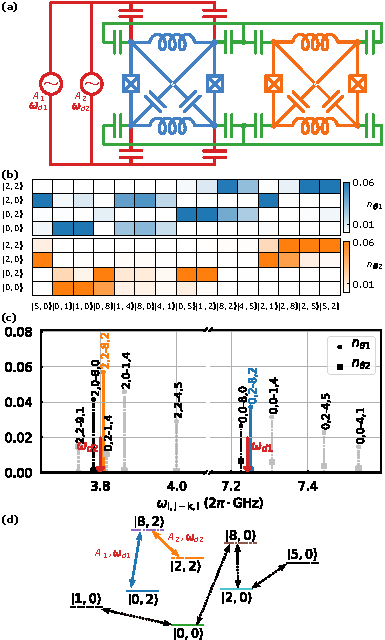
\includegraphics[width=\colfigwidth]{chapter-4-zero-pi/figs/cnot_ntheta.pdf}
\centering
\caption[CNOT gate implemented by driving $n_{\theta 1}$.]{   CNOT gate implemented by driving $n_{\theta 1}$.
(a) Circuit diagram.
The coupling and drive circuits are depicted in green and red, respectively.
(b) Charge matrix elements of $n_{\theta 1}$ and $n_{\theta 2} $ between two-qubit logical states and some non-logical states.
Note that the matrix elements used in the CNOT gate correspond to the $n_{\theta 1}$ matrix elements for the $\ket{2,2}$-$\ket{8,2}$ and $\ket{0,2}$-$\ket{8,2}$ transitions.
(c) Charge matrix elements $n_{\theta 1}$ and $n_{\theta 2}$ versus transition frequency $\omega_{i,j \text{-} k,l}$ for a transition $\ket{i,j}$-$\ket{k,l}$.
The two Raman transitions are depicted in blue and orange, while the two dominant leakage transitions are depicted in green and red.
(d) Energy level diagram.
The Raman and leakage transitions are plotted using the same color scheme as in panel (c).
}\label{zp:fig:cnot_ntheta}
\end{figure}

\subsection{Transition selection and gate principle}\label{zp:sec_sub:cnot_transition}

To identify a suitable Raman pathway, we examine the matrix elements of $n_{\theta 1}$ in \cref{zp:fig:cnot_ntheta}(b).
The rows correspond to computational states and the columns to low-energy non-computational states.
A column containing two appreciable matrix elements identifies a candidate intermediate state for an effective $\Lambda$ system.
Desirable pathways combine large matrix elements, which enable faster gates, with sufficient spectral isolation to suppress off-resonant transitions.

\Cref{zp:fig:cnot_ntheta}(c) shows the relevant matrix elements as a function of transition frequency.
Although the pathway through $\ket{4,5}$ is the most spectrally isolated, numerical optimization gives better gate performance using $\ket{8,2}$.
This indicates that spectral isolation alone does not determine the fidelity: the complete set of matrix elements, detunings, and off-resonant couplings must also be considered.
We therefore use $\ket{8,2}$ as the intermediate state.\footnote{The single-qubit $n_\theta$ gate involves $\ket{7}$.
In the coupled circuit, charging-energy renormalization produces an avoided crossing and exchanges the roles of $\ket{7}$ and $\ket{8}$, so that $\ket{8}$ plays the analogous role here.
See \cref{zp:sec:crossing}.}

The inter-qubit coupling spectrally separates the Raman pathways through $\ket{8,0}$ and $\ket{8,2}$, allowing the latter to be driven selectively.
Two tones couple $\ket{0,2}\leftrightarrow\ket{8,2}$ and $\ket{2,2}\leftrightarrow\ket{8,2}$, as shown in \cref{zp:fig:cnot_ntheta}(d).
The first qubit is therefore flipped only when the second qubit is in $\ket{2}$, implementing a CNOT with qubit 2 as the control and qubit 1 as the target.
Residual phases are removed using single-qubit $Z$ rotations, as shown in \cref{zp:sec:cnot_z_correction}~\cite{nesterov2022cnot}.

Other choices of Raman pathway produce different two-qubit gates.
Coupling $\ket{0,0}$ and $\ket{2,2}$ gives a bSWAP gate, while coupling $\ket{0,2}$ and $\ket{2,0}$ gives an iSWAP gate.

\subsection{Gate operation and noiseless fidelity}\label{zp:sec_sub:cnot_fidelity}
Panels (a)--(d) of \cref{zp:fig:cnot_population} show the noiseless time evolution of various two-qubit state populations during the CNOT.
The drive pulses are optimized in the same way as in the single-qubit case, with details given in \cref{zp:sec:2Qgate_simulation}.

The optimized gate has duration $t_{\rm g}=170$ ns and fidelity $F \sim 99\%$.
As expected, only cases where the control qubit is in $\ket{2}$ show population transfer at the final time, as seen in \cref{zp:fig:cnot_population}(b) and (d).
The intermediate state $\ket{8,2}$ is substantially populated, reaching $>40\%$.

From \cref{zp:fig:cnot_population}(a) and (c), we identify $\ket{8,0}$ as the dominant leakage state, from which we infer that the main leakage transitions are $\ket{0,0}$-$\ket{8,0}$ and $\ket{2,0}$-$\ket{8,0}$.
These are plotted in green and red in \cref{zp:fig:cnot_ntheta}(c) and (d).
The leakage during the CNOT gate is small, which can be deduced from the population in unintentionally populated states (``other'').
The total population in these states is approximately $0.66\%$, with no single state's contribution exceeding $0.15\%$.
This indicates only minimal leakage during the gate.

\begin{figure}[htbp]
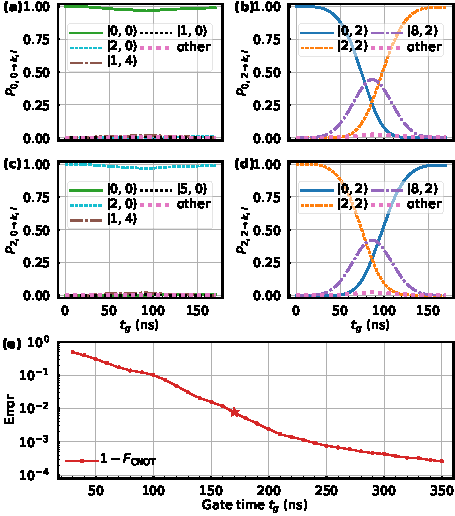
\includegraphics[width=\colfigwidth]{chapter-4-zero-pi/figs/cnot_combined.pdf}
\centering
\caption[Population transfer and error of the CNOT gate.]{Noiseless time evolution of the populations of various states during gate operation.
In subfigures (a)--(d),
the symbol $P_{i,j \rightarrow k,l }$ denotes the population transfer that starts at the state $\ket{i,j}$  and ends in the state $\ket{k,l}$.
The ``other'' state refers to the total population of all states not explicitly shown within the lowest 1000 dressed states.
(e) Average gate error ($1-F$) versus $t_g$ in the absence of noise.
Each point corresponds to optimized pulse parameters for the given $t_g$.
Star markers indicate the population transfer shown in (a)--(d).
}\label{zp:fig:cnot_population}
\end{figure}

Finally, \cref{zp:fig:cnot_population}(e) shows the average gate error ($1-F$) versus $t_g$ in the absence of noise.
Compared to the CZ gate discussed in the main text, this gate is much slower.
Similar to the single-qubit lambda gates, it also exhibits some leakage.
In principle, STIRAP could protect the gate, but competing factors such as decoherence arise.
Ultimately, the slow operation time is the main limitation.
For this reason we do not study decoherence for the CNOT gate.

Now we compare the CNOT gate with the CZ from the main text.
The CZ gate achieves both shorter duration and higher fidelity.
This advantage arises for two reasons: (i) CNOT requires driving two transitions in a $\Lambda$ system, while CZ uses direct transitions; and (ii) the relevant CZ transition has a charge matrix element an order of magnitude larger, with $\bra{2,0}n_{\theta 2}\ket{5,0}=0.537$ compared to $\bra{0,2}n_{\theta 1}\ket{8,2}=0.037$ and $\bra{2,2}n_{\theta 1}\ket{8,2}=0.057$ for CNOT (see \cref{zp:tab:parameter_cz} and \cref{zp:tab:parameter_cnot}).

\subsection{Single-qubit \texorpdfstring{$Z$}{Z} corrections for the CNOT gate}\label{zp:sec:cnot_z_correction}
For a bipartite Hilbert space $\mathcal{H}_1\otimes \mathcal{H}_2$, a controlled-NOT with control on subsystem $i$ and target on $j$ is denoted $\mathrm{CNOT}_{ij}$.
The ideal $\mathrm{CNOT}_{21}$ is
\begin{equation}
 \mathrm{CNOT}_{21}=   \begin{bmatrix}
        1 & 0 & 0 & 0\\
        0 & 0 & 0 & 1\\
        0 & 0 & 1 & 0\\
        0 & 1 & 0 & 0\\
    \end{bmatrix}.
\end{equation}
Our numerics yield a candidate gate $U_{\rm can}$ by projecting the simulated propagator (from the master equation) into the logical space.
We parameterize its principal matrix elements as $z_{ij}= |z_{ij}|e^{i\phi_{ij}}$ and denote the small error terms collectively by $y$.
The resulting form is
\begin{equation}
  {U}_{\rm can} =
 \begin{bmatrix}
  |z_{00}|e^{i\phi_{00}} & y & y & y \\
  y &  y & y & |z_{02}|e^{i\phi_{02}} \\
  y & y & |z_{20}|e^{i\phi_{20}} & y \\
  y & |z_{22}|e^{i\phi_{22}} & y & y
 \end{bmatrix}.
 \end{equation}
The elements $|z_{ij}|$ are equal to 1 in the ideal operator, and the phases $\phi_{ij}$ capture the phase accumulated in time evolution that must be corrected.

To facilitate a comparison between this operator and the ideal CNOT, we apply additional single-qubit $Z$ rotations $R_z(\phi)=\exp[-i \phi Z/2]=\mathrm{diag} [e^{-i\phi/2},e^{i\phi/2}]$ both before and after the gate,
\begin{equation}
{U_{\rm f}}
=\! e^{-i\phi_{\rm gb}}
[R_z(\phi_2) \otimes R_z(\phi_1) ]
\cdot {U}_{\rm can} \cdot [ R_z(\phi_3)\otimes I ] \, .
\end{equation}
Here, $\phi_{\mathrm{gb}} =\phi_{00} - (\phi_1 +\phi_2 +\phi_3 )/2 $ is a global phase.
To cancel out all phases of the key matrix elements, we solve linear equations to find the $R_z(\phi_i)$ rotation angles
\begin{equation}
\begin{aligned}
  \phi_1 &= \frac 12 \left(  \phi_{00} - \phi_{02} + \phi_{20} - \phi_{22}\right)\,,\\
  \phi_2 &=   \frac 12 \left(  \phi_{00} + \phi_{02} - \phi_{20} - \phi_{22}\right)\,,\\
  \phi_3 &= \frac 12 \left( \phi_{00} - \phi_{02} - \phi_{20} + \phi_{22}\right)\, \,.
  \end{aligned}
\end{equation}
After using those angles, we arrive at
\begin{equation}
  {U}_{\rm f} =
 \begin{bmatrix}
  |z_{00}| & y' & y' & y' \\
  y' &  y' & y' & |z_{02}| \\
  y' & y' & |z_{20}| & y' \\
  y' & |z_{22}| & y' & y'
 \end{bmatrix}\,,
 \end{equation}
where the entries denoted by $y'$ are complex numbers and satisfy $\left|y'\right| \ll 1$ in the high-fidelity limit.
We then compute the gate fidelity between $U_{\rm f}$ and the ideal $\mathrm{CNOT}_{21}$.
A similar derivation for a $\mathrm{CNOT}_{12}$ is presented in Ref.~\cite{nesterov2022cnot}.

\begin{figure}[htbp]
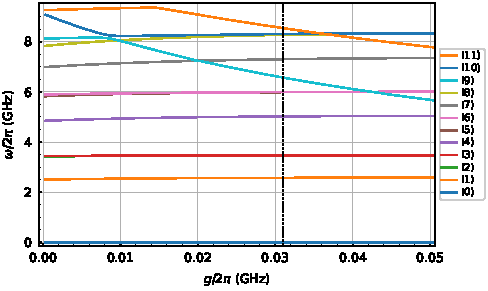
\includegraphics[width=\colfigwidth]{chapter-4-zero-pi/figs/eval_vs_g_full.pdf}
\centering
\caption[Level crossing versus coupling rate.]{
Energy spectrum of the first \zps qubit including coupling capacitances $C_c$ versus coupling rate $g$.
The black dashed line is the operating point of the coupled qubits, $g/2\pi \approx 0.031$ GHz.
Levels $\ket{7}$ and $\ket{8}$ cross near $g/2\pi \approx 0.02$ GHz.
}\label{zp:fig:crossing}
\end{figure}

\subsection{Level Crossing in Coupled Circuits}\label{zp:sec:crossing}
This section examines the level crossing between $\ket{7}$ and $\ket{8}$ as two \zps circuits are coupled.
\Cref{zp:fig:crossing} shows eigenvalues of the first \zps qubit versus coupling rate $g$, with $g=0$ for uncoupled systems.
Eigenvalue shifts arise solely from the renormalized charging energies in \cref{zp:eq:renormalized_ec}.
The coupling rate depends on the capacitance $C_c$ (\cref{zp:eq:coupling_rates_app}); larger $C_c$ yields stronger coupling.
For our gates, we use $E_{C_c}/h=1.0$ GHz (black dashed line), giving $g/2\pi\approx0.031$ GHz.

There are two important level crossings at  $g/2\pi \approx 0.01$ GHz, between $\ket{8}$ and $\ket{9}$, and at $g/2\pi \approx 0.02$ GHz, between $\ket{7}$ and $\ket{8}$.
These level crossings arise because the coupling capacitances renormalize the charging energies.
Because $\ket{7}$ is used as an intermediate state in the $X$ gate, we expect $\ket{7,2}$ to be an important candidate state for two-qubit gates when there is no level crossing.
However, due to the level crossing, $\ket{8,2}$ ends up being the intermediate state in the CNOT gate, while $\ket{7,2}$ has a nearly zero charge matrix element with respect to the logical states (not shown).
We therefore expect the best CNOT performance near $g/2\pi\approx0.031$ GHz.
This is the region where the intermediate state $\ket{8,2}$ is most isolated.

\begin{figure}[htbp]
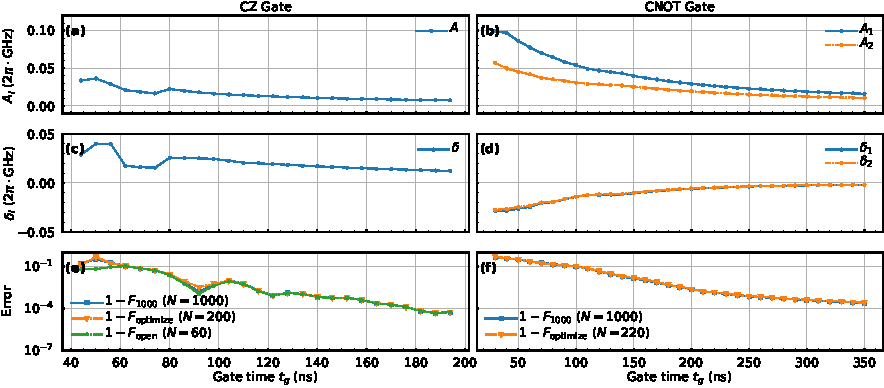
\includegraphics[width=\textwidth]{chapter-4-zero-pi/figs/params_2q.pdf}
\centering
\caption[Optimized two-qubit pulse parameters.]{
Optimized pulse parameters and gate infidelities for the CZ and CNOT gates.
For each gate time $t_g$, panels (a,b) show the optimized drive amplitude $A$, panels (c,d) show the optimized detuning $\delta$, and panels (e,f) show the corresponding infidelities.
For each fixed $t_g$, the Gaussian pulse is optimized in a truncated closed-system model of two coupled \zps qubits with $N_{\rm optimize}=200$ or $220$ selected levels, depending on the gate.
The resulting fidelity is $F_{\rm optimize}$.
The same optimized pulse is then tested in a closed-system model with $1000$ selected levels, giving $F_{1000}$,
and in a smaller ``selected'' $N$-level model, giving $F_{\rm open}$.
The ``selected'' $N$-level model is used for open-system simulation including energy relaxation and pure dephasing.
In this figure we only compare the closed-system fidelity for these three models.
Note that we were unable to simulate the CNOT gate in an open-system due to the large model needed for convergence ($N_{\rm open}=240$).
The plotted infidelities are $1-F_{\rm optimize}$, $1-F_{1000}$, and $1-F_{\rm open}$.
}\label{zp:fig:params_2q}
\end{figure}

\section{Two-Qubit Gate Simulation Details}\label{zp:sec:2Qgate_simulation}
The software used to generate the two-qubit gate simulation results is available in the repository \cite{zp2q_repo}.
This section provides a high-level overview of the numerical techniques used to simulate CZ and CNOT gates, along with key implementation details.
The goal is to help readers understand the core methods without requiring a deep dive into the source code.

\subsection{Noiseless simulation of two-qubit gates}
To simulate two-qubit gates, we first diagonalize the single-qubit Hamiltonians $H_{0\text{-}\pi}^{(1)}$ and $H_{0\text{-}\pi}^{(2)}$ to obtain eigenstates $\ket{p}^{(j)}$ and eigenvalues $E_p^{(j)}$, with $j = 1, 2$.
We retain the lowest 300 eigenstates for each qubit.
The eigenstates of the uncoupled system ($H_{\rm int} = 0$) are denoted $\ket{k}_0\otimes\ket{l}_0=\ket{k,l}_0$, where $k$ and $l$ label the eigenstates of the first and second qubits, respectively.

Next, we express the interaction term $H_{\rm int}$, e.g., $H_{\rm int}\approx  g_{\theta} n_{\theta_1}n_{\theta_2}$, in the uncoupled basis:
\begin{equation}
H_{\rm int} = \sum_{p,q,r,s=0}^{M_{\rm max}}
c_{pqrs}\, \ket{p}_0\bra{q} \otimes \ket{r}_0\bra{s},
\end{equation}
where $c_{pqrs} = g_\theta \,_0\bra{p,r} (n_{\theta 1}\otimes n_{\theta 2} )\ket{q,s}_0$.
We then diagonalize the full coupled Hamiltonian $H_{\rm cp} = H_{0\text{-}\pi}^{(1)} + H_{0\text{-}\pi}^{(2)} + H_{\rm int}$ to obtain dressed eigenstates $\ket{p, q}$ and eigenvalues $E_{p,q}$.
The resulting time-independent Hamiltonian $H_{\rm cp}$ is supplemented with a drive Hamiltonian and used to evolve the system under the Schr\"odinger equation:
\begin{equation}
i\frac{\partial V(t)}{\partial t} = \left( H_{\rm cp} + H_{\rm drive} \right) V(t).
\end{equation}
The evolution operator $V(t_g)$ at the final time $t_g$ is evaluated on the logical subspace spanned by $\{ \ket{0,0}, \ket{0,2}, \ket{2,0}, \ket{2,2} \}$ to form the $4 \times 4$ effective gate matrix $\bar V$, with elements
\begin{equation}
\bar V_{k,l;k',l'} = \bra{k,l} V(t_g) \ket{k',l'}.
\end{equation}
This operator is generally non-unitary due to leakage, although it will be nearly unitary for a high-fidelity operation.

\subsection{Noisy simulation of two-qubit gates} \label{zp:app:subsec_2Q_noise_details_and_converge}
We use a master equation with local (to each \zps system) energy relaxation ($L^r_{ij}$) and dephasing ($L^\varphi_l$).
The Lindblad operators for each \zps are constructed as
\begin{equation}\label{zp:eq:app_2Q_lindblad}
    \mathfrak{L}^{(1)} = L \otimes I\,\, {\rm and} \,\, \mathfrak{L}^{(2)} = I \otimes L\,,
\end{equation}
where $L \in \{L^r_{ij},\, L^\varphi_l\}$ and we have suppressed the indices needed to label all the operators.
Note that the operators in \cref{zp:eq:app_2Q_lindblad} are defined in the bare basis, but our simulations use the dressed basis.
These operators must be transformed into the dressed basis before solving the master equation.

Due to computational limitations, we cannot compute the noisy dynamics for systems with more than approximately 150 levels.
As seen in \cref{zp:fig:params_2q}, we identify a subset of states (60 for the CZ gate) that accurately represents the coherent dynamics of these operations.
As in the single-qubit gate case, we evolve the system in these reduced subspaces to obtain the propagator $e^{\mathcal{L} t}$  that maps the initial density matrix $\rho(0)$ to $\rho(t)$.
The resulting superoperator is projected into the computational subspace and corrected with single-qubit $Z$ rotations.
Finally, we compute the  average channel fidelity with the target CZ, according to \cref{zp:eq:channel_fidelity}.

 \section{Sensitivity Analysis of Circuit Parameters}\label{zp:app:sensitivity}

\begin{table}[htbp]
\centering
\setlength{\tabcolsep}{11pt}
\renewcommand{\arraystretch}{1.1}
\small
\begin{tabular}{ccc}
\toprule
\multirow{2}{*}{Parameter}
& \multicolumn{2}{c}{Sensitivity (decades)} \\
\cmidrule(lr){2-3}
& $t_g = 92~\mathrm{ns}$ & $t_g = 182~\mathrm{ns}$ \\ \midrule
$E_{C}$                 & 0.445  & 0.244  \\
$E_{CJ}$                & 0.000  & 0.000 \\
$E_{J}$                 & 0.549  & 0.336  \\
$E_{L}$                 & 0.242  & 0.000  \\
$E_{Cc}$ (coupling)      & 0.000  & 0.075  \\
$E_{C0}$ (ground)        & 0.000  & 0.000  \\
$\phi_{\mathrm{ext}}$  & 0.010  & 0.002  \\
$n_{g}^\theta$                & -0.001 & -0.001 \\
\bottomrule
\end{tabular}
\caption[Sensitivity of the CZ gate to parameter variations.]{
Robustness of the optimized CZ gates against fabrication-induced parameter variations and operating-point offsets.
Each circuit parameter of the second 0-$\pi$ qubit is independently varied by $\pm5\%$ around its nominal value while all other parameters are held fixed.
For circuit parameters, we take 21 uniformly sampled points for the statistics.
The offset parameters $n_{g}^{\theta}$ and $\phi_{\mathrm{ext}}$ are sampled uniformly in log-space over
the ranges $[10^{-6},10^{-2}]$ and $[10^{-8},10^{-4}]$, respectively.
The sensitivity is the median change in coherent gate error, measured in decades relative to the nominal-point gate error.
Negative values indicate that the median gate error over the sweep is slightly smaller than the nominal-point error.
Both optimized gates are robust against most fabrication variations, while the shorter 92-ns gate exhibits increased sensitivity to variations in $E_{C}$, $E_{J}$, and $E_{L}$.
}
\label{zp:tab:cz_sensitivity}
\end{table}

In this section, we investigate the robustness of the optimized gates against circuit-parameter variations and operating-point offsets.
Each circuit parameter of the second \zps qubit is sampled uniformly in a range $\pm5\%$ around its nominal value, while all other parameters are held fixed.
Note that the offset parameters $n_{g}^{\theta}$ and $\phi_{\mathrm{ext}}$ are sampled uniformly in log-space over the ranges $[10^{-6},10^{-2}]$ and $[10^{-8},10^{-4}]$, respectively.
The pulse is then re-optimized, and the corresponding coherent gate error is evaluated.
We use 21 points to generate the statistics in \cref{zp:tab:cz_sensitivity}.

We examine the two pulses highlighted in \cref{zp:fig:2q_fidelity}, whose parameters are summarized in \cref{zp:tab:parameter_cz}.
The shorter pulse, with $t_g\approx92$ ns, lies near a sharp minimum in the gate-error curve and is therefore expected to be sensitive to variations in gate time and other parameters.
By contrast, the $182$-ns pulse is not in a minimum, suggesting greater robustness to such variations.

The results are summarized in \cref{zp:tab:cz_sensitivity}.
The reported sensitivity is defined as the median value of $\log_{10}[(1-F)/(1-F_0)]$ over the parameter sweep, where $F_0$ is the coherent fidelity at the nominal parameter point; thus, one decade corresponds to a tenfold increase in coherent gate error.
The 182-ns gate is generally insensitive to these variations, with all parameters producing a median increase in coherent gate error of less than one order of magnitude.
By contrast, the faster 92-ns gate is more sensitive to variations in $E_{C}$, $E_{J}$, and $E_{L}$, while remaining comparatively robust against changes in $E_{CJ}$, $\phi_{\mathrm{ext}}$, $n_{g}^{\theta}$, the coupling energy $E_{Cc}$, and the ground-capacitance energy $E_{C0}$.
These results demonstrate the trade-off between gate speed and robustness, with the longer gate exhibiting substantially improved tolerance to parameter variations.
